\documentclass[tikz]{standalone}
\usetikzlibrary{arrows.meta, bending, decorations.markings, positioning, shapes}

\begin{document}

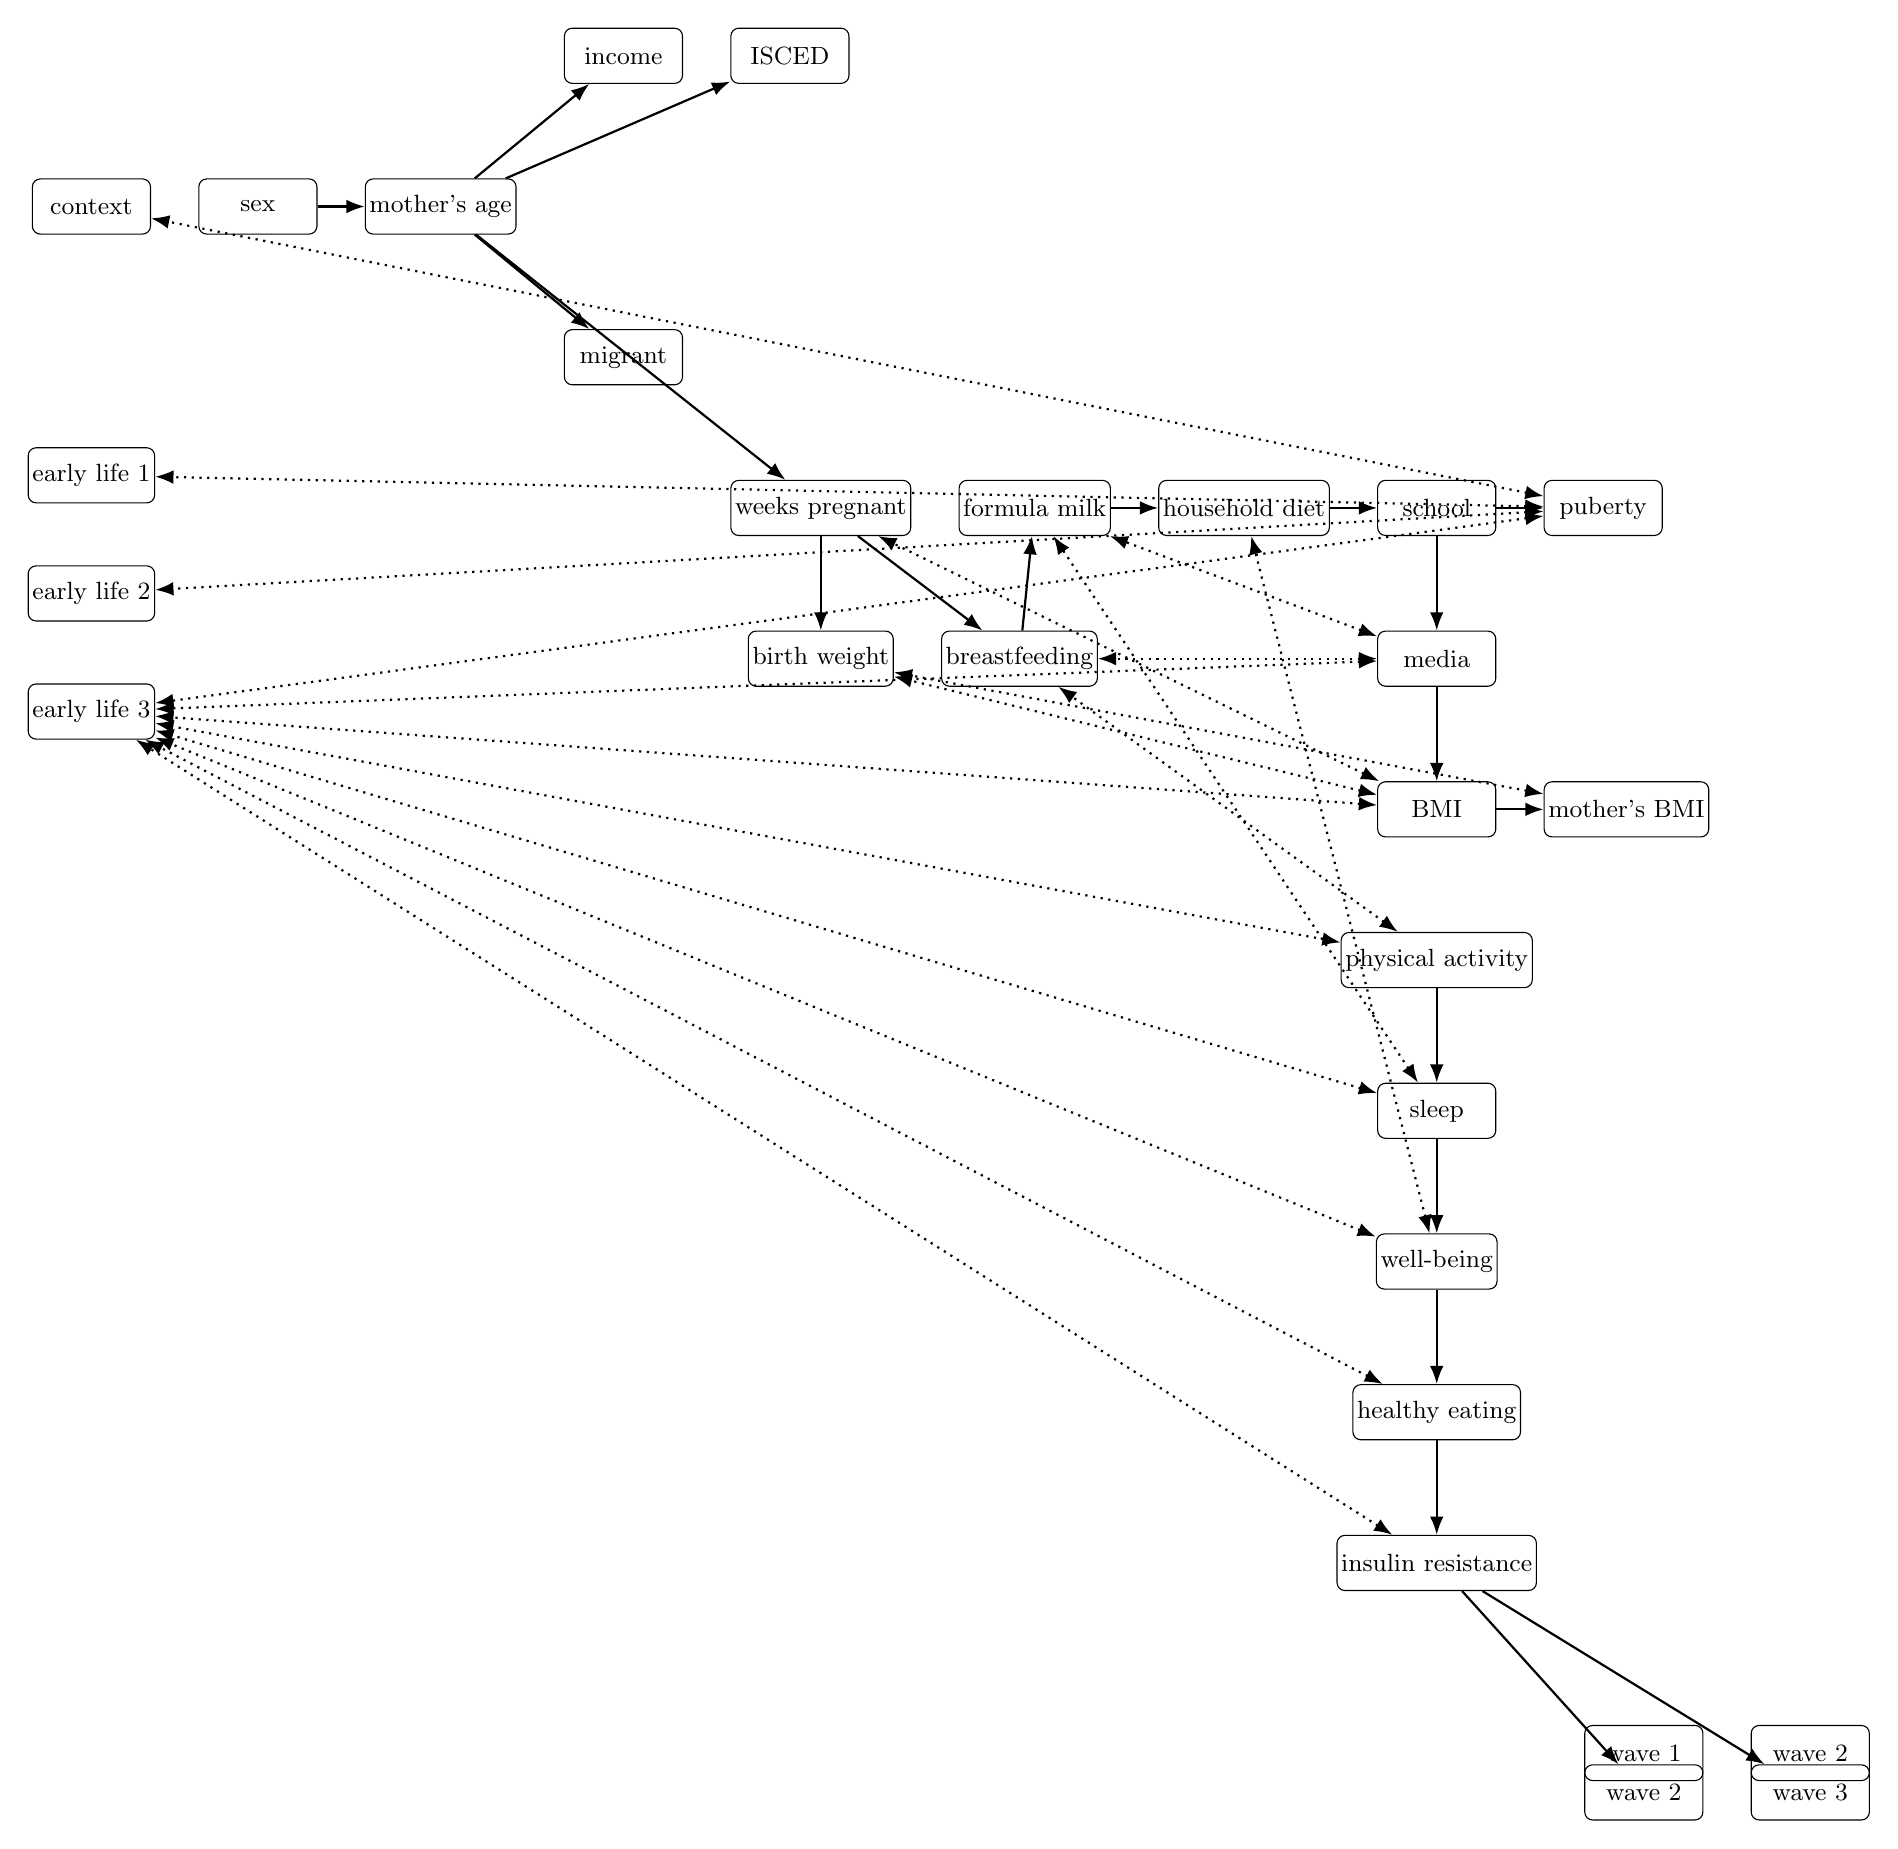
\begin{tikzpicture}[
    -Latex, auto,
    node distance = 12mm and 6mm,
    every label/.style = {font =\small},
    cnode/.style = {draw=none, minimum height=4mm, minimum width=4mm},
    snode/.style = {draw, rounded corners=0.1cm, inner sep=1.5pt, minimum height=0.7cm, minimum width=1.5cm, font=\small},
    eline/.style={-Latex, thick},
    tline/.style={Latex-Latex, dotted, thick}
    ]

% Nodes
\node[snode] (sex) {sex};
\node[snode, right=of sex] (m_age) {mother's age};
\node[snode, above right=of m_age] (income) {income};
\node[snode, below right=of m_age] (migrant) {migrant};
\node[snode, right=of income] (ISCED) {ISCED};

% Early life nodes
\node[snode, below right=of migrant] (w_preg) {weeks pregnant};
\node[snode, below=of w_preg] (b_weight) {birth weight};
\node[snode, right=of w_preg] (formula) {formula milk};
\node[snode, right=of formula] (h_diet) {household diet};
\node[snode, right=of b_weight] (breast) {breastfeeding};

% Baseline nodes
\node[snode, right=of h_diet] (school) {school};
\node[snode, below=of school] (media) {media};
\node[snode, below=of media] (bmi) {BMI};
\node[snode, right=of school] (puberty) {puberty};
\node[snode, right=of bmi] (m_bmi) {mother's BMI};
\node[snode, below=of bmi] (p_activity) {physical activity};
\node[snode, below=of p_activity] (sleep) {sleep};
\node[snode, below=of sleep] (wellbeing) {well-being};
\node[snode, below=of wellbeing] (h_eating) {healthy eating};
\node[snode, below=of h_eating] (insulin) {insulin resistance};

% Waves
\foreach \i/\j in {1/2, 2/3} {
    \node[snode, below right=of insulin, yshift=-0.5cm*\i] (wave\i) {wave \i};
    \node[snode, right=of wave\i] (wave\j) {wave \j};
}

% Context and early life
\node[snode, left=of sex] (context) {context};
\foreach \i in {1,2,3} {
    \node[snode, below=of context, yshift=-1.5cm*\i] (early\i) {early life \i};
}

% Edges
% Bold edges (expected)
\draw[eline] (sex) to (m_age);
\draw[eline] (m_age) to (migrant);
\draw[eline] (m_age) to (income);
\draw[eline] (m_age) to (ISCED);
\draw[eline] (m_age) to (w_preg);
\draw[eline] (w_preg) to (b_weight);
\draw[eline] (w_preg) to (breast);
\draw[eline] (breast) to (formula);
\draw[eline] (formula) to (h_diet);
\draw[eline] (h_diet) to (school);
\draw[eline] (school) to (puberty);
\draw[eline] (school) to (media);
\draw[eline] (media) to (bmi);
\draw[eline] (bmi) to (m_bmi);
\draw[eline] (p_activity) to (sleep);
\draw[eline] (sleep) to (wellbeing);
\draw[eline] (wellbeing) to (h_eating);
\draw[eline] (h_eating) to (insulin);
\foreach \i/\j in {1/2, 2/3} {
    \draw[eline] (insulin) to (wave\j);
}

% Dotted edges (implausible)
\draw[tline, dotted] (puberty) to (context);
\draw[tline, dotted] (puberty) to (early1);
\draw[tline, dotted] (puberty) to (early2);
\draw[tline, dotted] (puberty) to (early3);
\draw[tline, dotted] (m_bmi) to (b_weight);
\draw[tline, dotted] (media) to (early3);
\draw[tline, dotted] (media) to (breast);
\draw[tline, dotted] (media) to (formula);
\draw[tline, dotted] (bmi) to (early3);
\draw[tline, dotted] (bmi) to (w_preg);
\draw[tline, dotted] (bmi) to (b_weight);
\draw[tline, dotted] (p_activity) to (early3);
\draw[tline, dotted] (p_activity) to (breast);
\draw[tline, dotted] (sleep) to (early3);
\draw[tline, dotted] (sleep) to (formula);
\draw[tline, dotted] (wellbeing) to (early3);
\draw[tline, dotted] (wellbeing) to (h_diet);
\draw[tline, dotted] (h_eating) to (early3);
\draw[tline, dotted] (insulin) to (early3);

\end{tikzpicture}
\end{document}